\section{Translator Architecture (\textit{Marcin})}

\subsection{Architectural Block Diagram of the Translator}

The SwiftFox compiler architecture consists of four phases, namely 
lexical analysis, syntax analysis, intermediate code generator, and target 
nesC code generator. Figure \ref{fig:arch} depicts all the phases of the
SwiftFox compiler.

\begin{figure}[htp]
\centering
        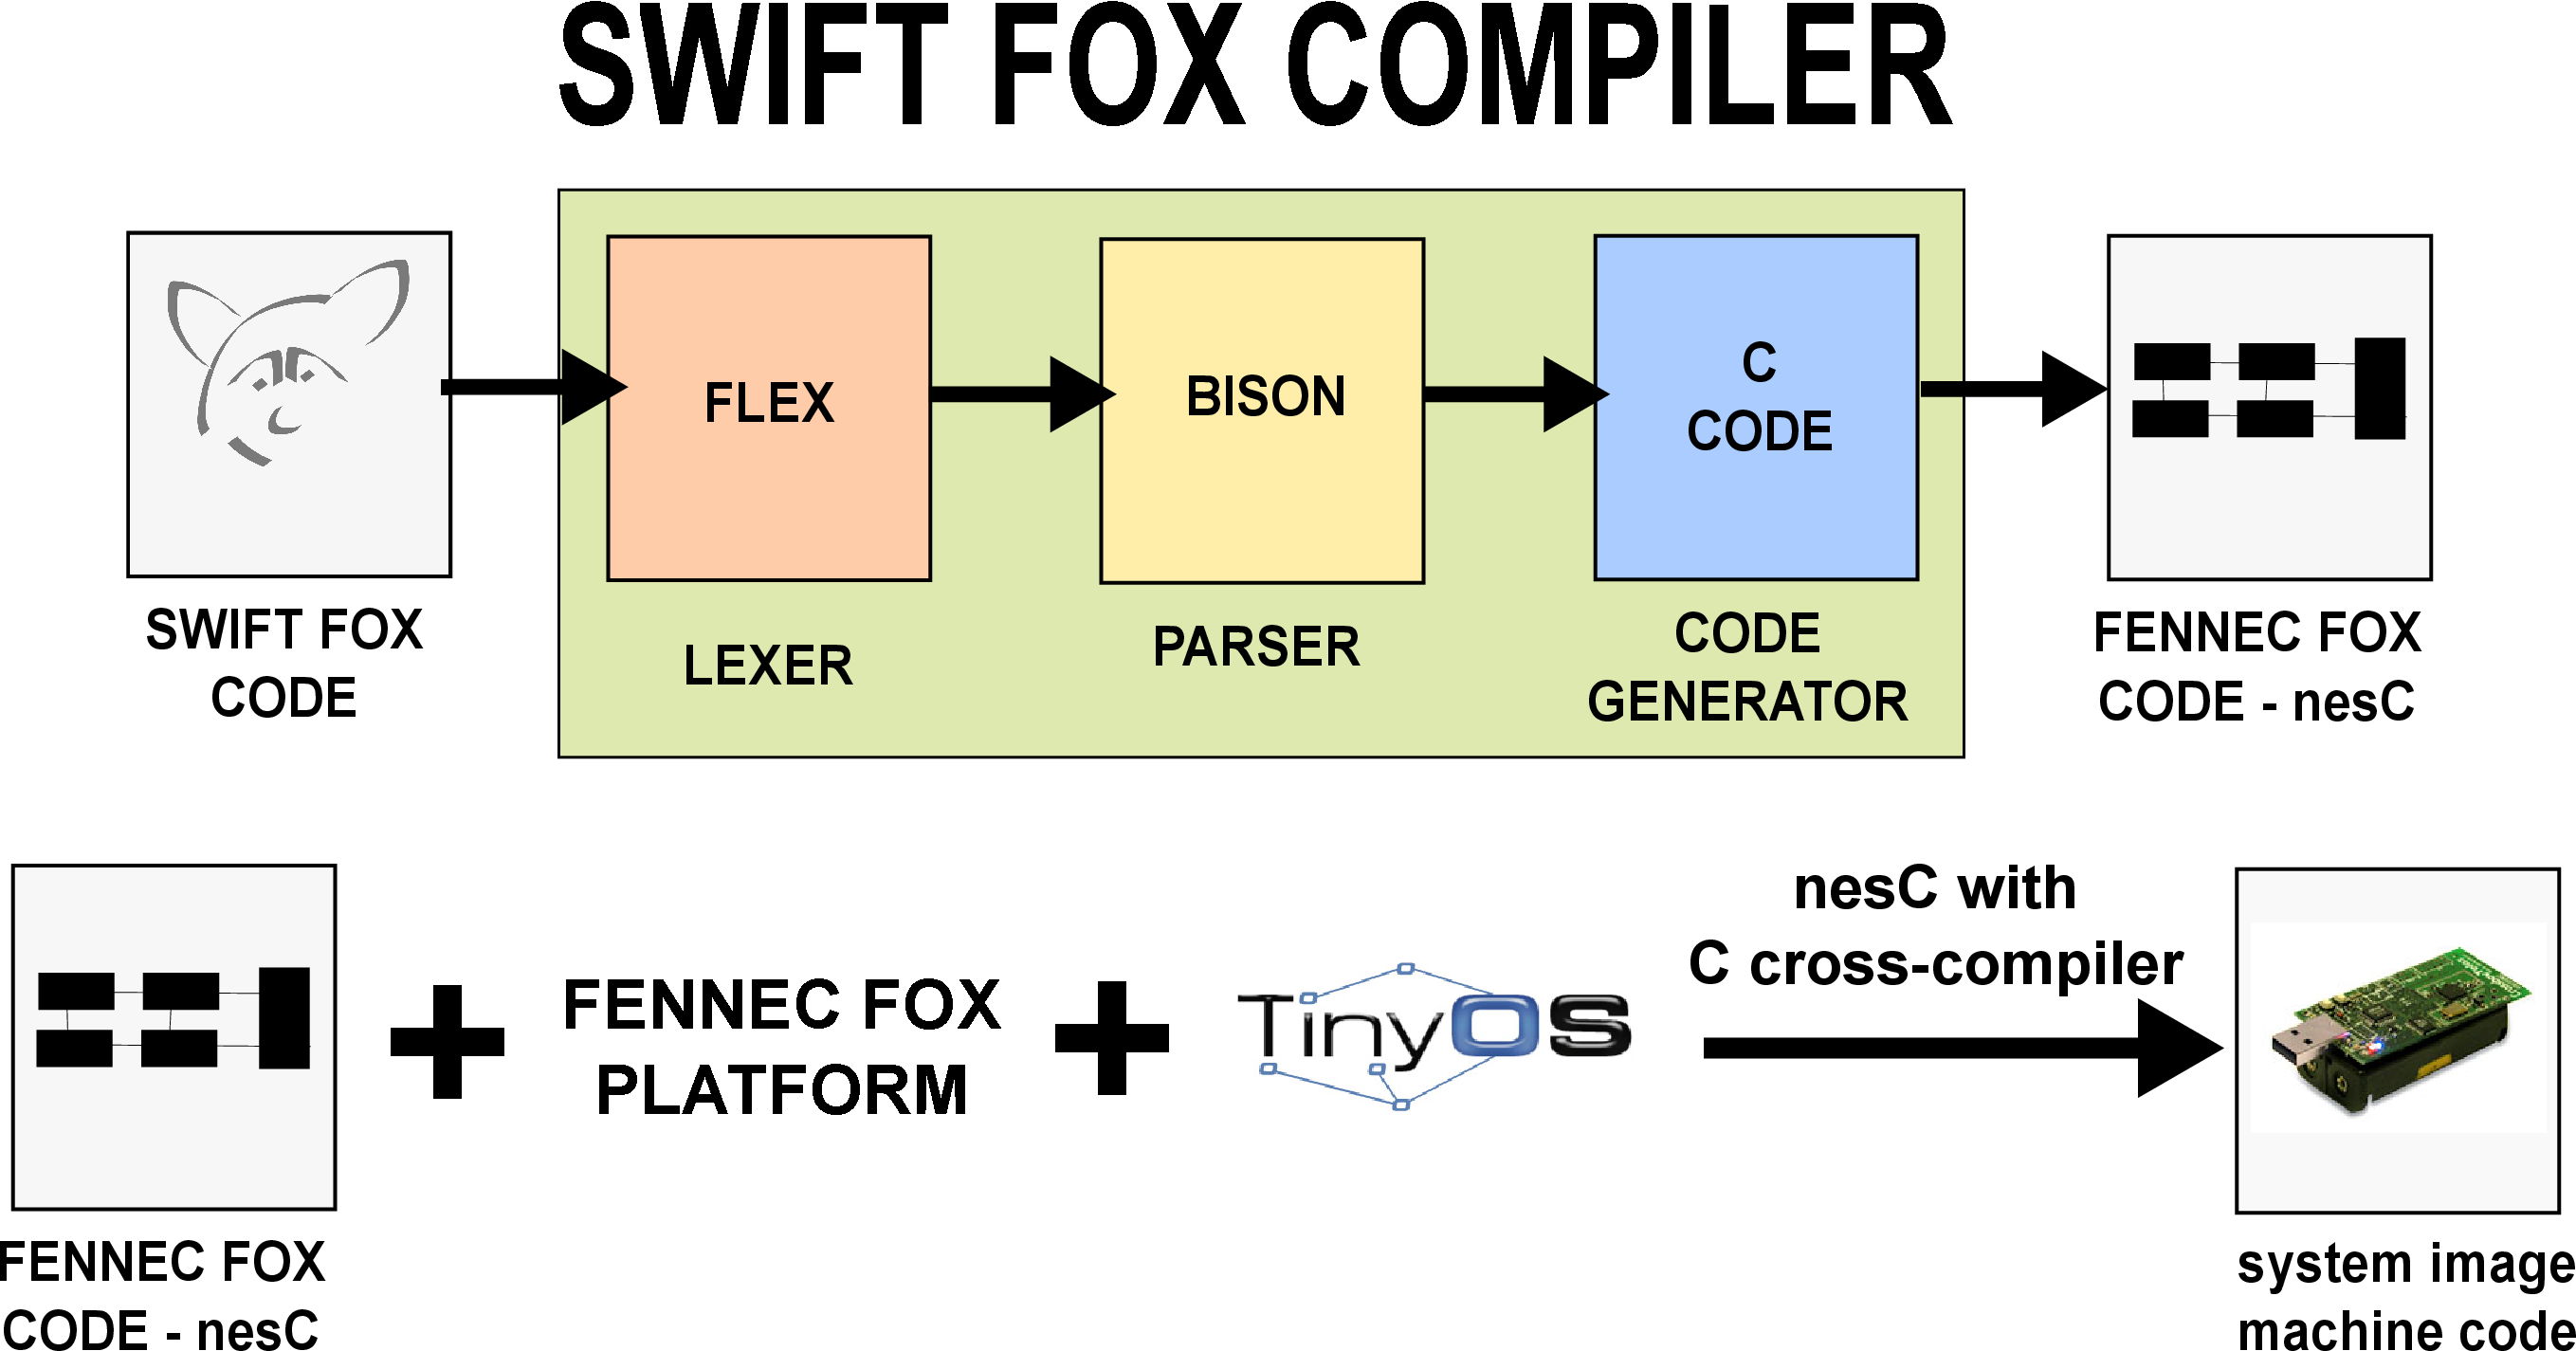
\includegraphics[scale=0.12]{fig/arch.eps}
        \caption{Swift Fox compiler architecture.}
        \label{fig:arch}
\end{figure}

\subsection{Modules and Interfaces}

First, the lexical analyzer receives a stream of characters from two 
files:\textit{i.} a library file, and \textit{ii.} a program code file. The
library file specifies what libraries are accessible to the program code,
and where they are located. The program code file contains code that
implements configurations, events, and policies. The lexical analyzer was
implemented using flex \cite{paxson:2010} and saved in \texttt{sf.l} file. 
Besides tokenizing the input text, the lexical analyzer also implements
debug code used to verify correctness of the lexer functionality, and also 
keeps track of the text that is tokenized to be able to return helpful
error messages.

Second, the syntax analyzer receives the stream of tokens from 
the lexical analyzer. All terminals and non-terminals are 
defined in the syntax analyzer which was implemented using
bison \cite{bison:2010} and saved in \texttt{sf.y} file. As the syntax
analyzer is parsing the input, it uses synthesized attributes to create
annotated parse tree. The generated parse tree fills out all necessary information
for the further semantic check and code generation processes.
These information are related to types, values, and links to
the libraries that provide the requested functionality. The parser
also tracks how much memory is necessary to be reserved for the
code generated by the compiler. The memory management done
by the parser is critical to insure that the final machine
code will required minimum of ROM space, particularly because it 
is to be deployed on small embedded devices. 

Third, the parse tree generated by the syntax analyzer is traversed
twice for semantic checking and for code generation. The semantic check
was not fully implemented as we expected. During the code generation
the parse tree is traversed and code is generated and stored in files
which are part of the Fennec Fox platform. The Swift Fox code generation
creates 10 files which are part of the Fennec Fox and contain
code written in nesC. The code generation functionality was saved
in \texttt{code\_gen.c} and \texttt{code\_gen.h} files.

\subsection{Members Impact on the Architecture}

\begin{enumerate}

\item \textbf{Lexer}: Marcin and Vasileios
\item \textbf{Parser}: Marcin 
\item \textbf{Tree Traversal}: Yiwei (adapted to the parse tree by Marcin)
\item \textbf{Semantic Check}: Vasileios (after it was attempted by Linh)
\item \textbf{Code Generation}: Marcin
\item \textbf{Test Suite}: Vasileios (after it was attempted by Linh) 

\end{enumerate}
